\item Een doos van $10\rm\,kg$ wordt met een kracht van $40\rm\,N$ over een glad tafeloppervlak getrokken. De uitgeoefende kracht maakt een hoek van $30^\circ$ met de horizontaal. Als de wrijving mag worden verwaarloosd, bepaal dan
\newline
%\begin{figure}[h]
%\begin{center}
%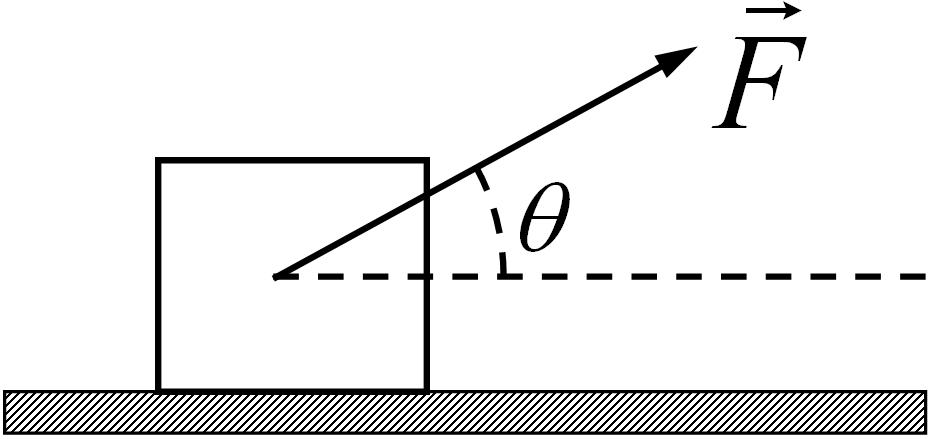
\includegraphics[width=0.4\textwidth]{doos_kracht}
%\end{center}
%\end{figure}
%\newline
%
%
\begin{minipage}[t]{.6\linewidth}
\begin{enumerate}
\item de versnelling van de doos,
\item de grootte van de normaalkracht, die de tafel op de doos uitoefent.
\end{enumerate}
\end{minipage}
\begin{minipage}[t]{.4\linewidth}
\vtop{%
  \vskip-1ex
  \hbox{%
    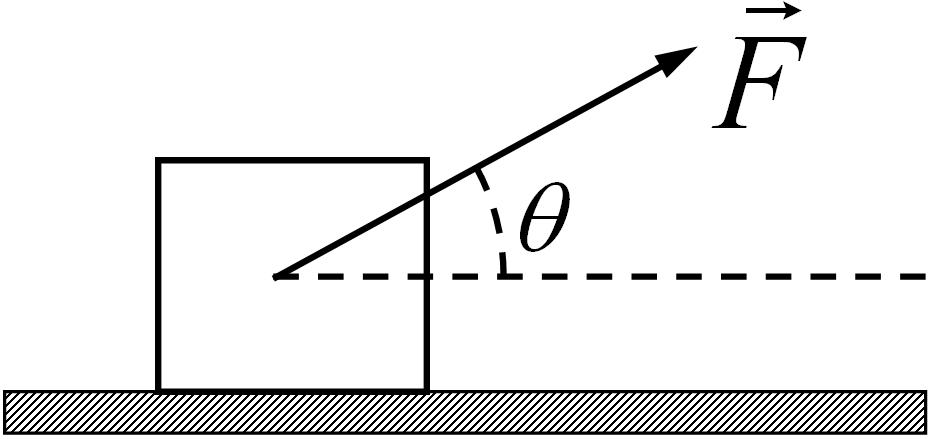
\includegraphics[width=\linewidth]{doos_kracht}%
  }%
}
\end{minipage}
%
%
%
%Als de wrijving mag worden verwaarloosd, bepaal dan
%\begin{enumerate}
%\item de versnelling van de doos,
%\item de grootte van de normaalkracht, die de tafel op de doos uitoefent.
%\end{enumerate}
\begin{oplossing}
\begin{enumerate}
\item $a=\frac{F\cos\theta}{m}=3,46\rm\,m/s^2$
\item $F_n=mg-F\sin\theta=78,1\rm\,N$
\end{enumerate}
\end{oplossing}
